\documentclass[12pt]{article}

\usepackage{amsmath}
\usepackage{amssymb}
\usepackage{amsthm}
\usepackage{graphicx}
\usepackage{float}

\title{An Introduction To\\Conformal Geometric Algebra}
\author{Spencer T. Parkin}

\newcommand{\G}{\mathbb{G}}
\newcommand{\V}{\mathbb{V}}
\newcommand{\R}{\mathbb{R}}
\newcommand{\B}{\mathbb{B}}
\newcommand{\nvao}{o}
\newcommand{\nvai}{\infty}

\newtheorem{theorem}{Theorem}[section]
\newtheorem{definition}{Definition}[section]
\newtheorem{corollary}{Corollary}[section]
\newtheorem{identity}{Identity}[section]
\newtheorem{lemma}{Lemma}[section]
\newtheorem{result}{Result}[section]

\begin{document}
\maketitle

\begin{abstract}
The conformal model of geometric algebra is set forth.
Its development here proceeds apart from many other treatments
of the subject, mainly by requiring more rigor where it is common
to give features of the model without proof. Questions arising
in the model are considered, as well as a possible extension to the model.
\end{abstract}

Conformal geometric algebra (CGA) is a model of
geometry implemented in the language of geometric algebra.
This document is my attempt to rigorously build the
conformal model from the ground up, as well as to explore
arising questions in the model and even consider a reasonable
extension of the model.
It is only assumed that the reader is familiar with geometric algebra.
The books $\cite{dorst07}$ and $\cite{hestenes87}$ were
used most by the author in the preparation of this document.
I recommend them for further study along with the other resources
found in the reference section.

All 3-dimensional figures given in this paper were generated
by a piece of prototype software developed by the author named GAVisTool,
but the reader should be made aware
of better tools for studying CGA such as GAViewer
and CLUCalc, both of which can be easily found on the internet.

\nocite{zaharia02}
\nocite{hildenbrand05}

\section{Representing Geometry}

We begin by defining how geometries are represented in the model.
Letting $\R^n$ denote $n$-dimensional Euclidean space, we will
represent geometries as subsets of this space.  Having done so,
we may perform unions, intersections and other operations of geometries, but we
have no easy means of performing any geometric analysis.  Measurements, normals,
tangents, centers, shape and other things that may characterize a geometry are not
so easily gleaned or inferred from a set of points.  This is where
geometric algebra comes in.

Letting $\G$ denote the geometric algebra to be used by our model
of geometry, we begin by letting $p:\R^n\to\G$ be a vector-valued
function of a Euclidean point, the definition of which we leave
open for the moment.  We then use this function in the following definition.
\begin{definition}\label{def_direct_rep}
For any blade $B\in\G$, we say that $B$ directly
represents a geometry as the set of points
$G(B)=\{x\in\R^n|p(x)\in B\}$.
\end{definition}
Recall that for any vector $v\in\G$, we say that $v\in B$ if and only if $v\wedge B=0$.
Clearly this means that $v$ is in the vector space spanned by any vector factorization
of $B$.  Letting $B^*$ denote a dual of $B$, it is not hard to show that
$v\in B^*$ if and only if $v\cdot B=0$.
\begin{definition}\label{def_dual_rep}
For any blade $B\in\G$, we say that $B$ dually
represents a geometry as the set of points
$G^*(B)=\{x\in\R^n|p(x)\in B^*\}$.
\end{definition}
Notice that by any one of these two definitions, if $B$ represents
a given geometry, then so does $B^*$ by the other definition.
That is, $G(B)=G^*(B^*)$ and $G^*(B)=G(B^*)$.
Furthermore, any non-zero scalar multiple of $B$ is also representative
of the same geometry.  That is, for all non-zero $\lambda\in\R$,
we have $G(B)=G(\lambda B)$.  This illustrates the homogeneity of
our representation scheme.

\section{Operations of Geometry}

Noticing that the set of all blades in $\G$ is closed under the
outer product operation of geometric algebra,
a natural question arises as to what geometries are represented
by the results of this operation in terms of
the geometries directly or dually represented by its operands.  To begin to answer this,
we start with a theorem.
\begin{theorem}\label{thm_intersect}
For any vector $v\in\G$ and any two blades $A,B\in\G$,
if $A\wedge B\neq 0$, then $v\cdot A=0$ and $v\cdot B=0$ if and only if $v\cdot A\wedge B=0$.
\end{theorem}
\begin{proof}
If $A\wedge B\neq 0$, then $A\wedge B$ represents the union of the vector sub-spaces
represented by $A$ and $B$.  Stating the next part of the theorem another way, we can
say that $v\wedge AI=0$ and $v\wedge BI=0$ if and only if $v\wedge (A\wedge B)I=0$,
which is also to say that $v\not\in A$ and $v\not\in B$ if and only if $v\not\in A\wedge B$.
\end{proof}
If $A\wedge B=0$, then the calculation of the union of the vector sub-spaces represented by
$A$ and $B$ is a bit more involved, but is a more general formula for what we call the join
of $A$ and $B$.  The meet operation gives us the blade representative of the intersection
of the represented vector sub-spaces. The more general meet and join
operations may have their uses in the conformal model, but here, for simplicity, we will stick to the
simpler case of the join operation.

We can apply theorem $\eqref{thm_intersect}$ to get the following result.
\begin{result}\label{rslt_intersect}
For any two blades $A,B\in\G$ such that $A\wedge B\neq 0$, we have
\begin{equation*}
G^*(A)\cap G^*(B) = G^*(A\wedge B).
\end{equation*}
\end{result}
Interestingly, we see here that the outer product gives the
dual representation of the intersection between the two geometries
dually represented by the blades taken in that product.
\begin{theorem}\label{thm_union_and_more}
For any vector $v\in\G$ and any two blades $A,B\in\G$,
if $v\wedge A=0$ or $v\wedge B=0$, then $v\wedge A\wedge B=0$.
\end{theorem}
\begin{proof}
If $A\wedge B=0$, then we're done.  If $A\wedge B\neq 0$ and $v\in A$ or $v\in B$,
then $v\in A\wedge B$, which is to say that $v$ is in the union of the vector sub-spaces
represented by $A$ and $B$.
\end{proof}
To see why the converse of theorem $\eqref{thm_union_and_more}$ does not generally hold,
realize that if $v\in A\wedge B$, then the vector sub-space of $A\wedge B$ of smallest dimension
containing $v$ might non-trivially overlap both $A$ and $B$, showing that $v\not\in A$ and
$v\not\in B$.

Applying theorem $\eqref{thm_union_and_more}$, we get the following result.
\begin{result}\label{rslt_union_and_more}
For any two blades $A,B\in\G$, we have
\begin{equation*}
G(A)\cup G(B)\subseteq G(A\wedge B).
\end{equation*}
\end{result}
Here we see that the outer product gives the direct representation
of a geometry that is at least the union of the geometries directly
represented by the blades taken in that product.  Unlike the intersection
result given earlier, however, here we cannot come to any certain conclusion
about what is being represented, even if we know exactly what
geometries are being represented by the operands of the operation.
To resolve this, we'll find a relationship between the geometries
generated through the use of the intersection operation and the geometries
generated through the use of the union-like operation.

\section{Generating Geometry}

Having not yet defined the function $p(x)$ or the signature of our
geometric algebra $\G$, what we have covered so far applies to
any number of possible models of geometry based upon geometric algebra.
Therefore, to start getting specific about geometry in the conformal model,
we will now give an explicit formula for $p(x)$ and define $\G$.
As part of this, we will embed $\R^n$ in $\G$.  Notice, however, that
this is not a requirement of the generalized model, but it is how
the conformal model works.
We do this by replacing $\R^n$
with an $n$-dimensional Euclidean vector space $\V^n$, (interpreting
Euclidean vectors as Euclidean points in the usual manner), and
make the geometric algebra generated by this vector space
a sub-algebra of $\G$.\footnote{To avoid any further pedanticism in this paper than will already be encountered,
we will refer to vectors in $\V^n$ informally as Euclidean points or Euclidean vectors at will.}
Specifically, if $\{e_k\}_{k=1}^n$ is
any set of $n$ basis vectors for $\V^n$, then a set of
basis vectors for a vector space we'll denote by $\V$ generating $\G$
is given by $\{\nvao,\nvai\}\cup\{e_k\}_{k=1}^n$, where $\nvao$ and $\nvai$ are
referred to as the null vectors
at the origin and infinity, respectively.
\begin{definition}
For any vector $v\in\V$, if $v\cdot v=0$, we call $v$ a null vector.
\end{definition}
The null vectors $\nvao$ and $\nvai$ obey the relationship
$\nvai\cdot\nvao=-1$.  Furthermore, for
all vectors $v\in\V^n$, we define $v\cdot\nvao=0$ and $v\cdot\nvai=0$.

Having precisely defined our geometric algebra $\G$, we define
$p:\V^n\to\G$ as follows.
\begin{equation*}
p(x) = \nvao + x + \frac{1}{2}x^2\nvai
\end{equation*}
It is now not hard to show that for any $x\in\V^n$, the vector $p(x)$
both directly and dually represents the Euclidean point $x$.  We leave
this as an exercise
for the reader, as well as showing that for any scalar $r>0$, that
$p(x)-\frac{1}{2}r^2\nvai$ dually represents an $n$-dimensional hyper-sphere
at $x$ with radius $r$.  The reader should also convince themselves that a
vector of the form $v+(x\cdot v)\nvai$ dually represents an $(n-1)$-dimensional
hyper-plane containing the
point $x$ and being orthogonal to the unit-normal $v\in\V^n$.

Now having blades that represent the spheres and planes in the highest possible
dimensions of interest in $n$-dimensional Euclidean space, let us now apply
the intersection result $\eqref{rslt_intersect}$ to generate as many round
and flat geometries as we can.  Doing so, we see that we can generate
hyper-spheres and hyper-planes of dimensions $0$ through $n-1$ as
outer products of vectors.  For $n=3$, the following table summarizes
the geometries we find and the grades of the blades dually representing them.
\begin{equation*}
\begin{array}{ccccccc}
\mbox{Grade} & \vline & \mbox{Degenerate Dual Round} & \vline & \mbox{Dual Round} & \vline & \mbox{Dual Flat} \\
\hline
1 & \vline & \mbox{Point} & \vline & \mbox{Sphere} & \vline & \mbox{Plane} \\
2 & \vline & \mbox{Tangent-Point} & \vline & \mbox{Circle} & \vline & \mbox{Line} \\
3 & \vline & \mbox{Tangent-Point} & \vline & \mbox{Point-Pair} & \vline & \mbox{Flat-Point}
\end{array}
\end{equation*}
There is nothing more or less that characterizes a flat-point in comparison
to a regular point, which may be thought of as a round-point, also being
a degenerate sphere (a sphere of radius zero).  Flat-points are called flat,
because they're the first entry in the list of flat geometries in order of
increasing dimension.  (Flat-point, line, plane, hyper-plane, etc.)

At first glance, the point-pair may seem out-of-place, but it is simply
the 1-dimensional analog of a sphere or circle.  It has a center and
a radius, but only two points.

The dual tangent point of grade 2 is a degenerate
circle, and the dual tangent point of grade 3 is a degenerate point-pair.
These occur when we intersect a plane in one point on a round,
which is why they're called tangent points.

Using the intersection result $\eqref{rslt_intersect}$ with $n$-dimensional hyper-spheres
and $(n-1)$-dimensional hyper-planes, we come to the following result relating the grade of a blade
with the geometry dually represented by that blade.
\begin{result}\label{rslt_intersect_grades}
If $B\in\G$ is a blade dually representative of an $m$-dimensional
hyper-sphere, then the grade of $B$ is $n-m+1$.  If $B\in\G$ is a blade
dually representative of an $m$-dimensional hyper-plane, then the
grade of $B$ is $n-m$.
\end{result}

A close look at the vector forms of $n$-dimensional hyper-spheres and $(n-1)$-dimensional
hyper-planes will reveal that we have exhausted all the types of geometries that we can
represent using a vector.  (Imaginary spheres will be treated in a later section.)
Let us now turn our attention to the method of generating
geometries using the union-like result $\eqref{rslt_union_and_more}$.  Interestingly, what we'll
find is that we can generate the above geometries using this method.
We start with a definition.
\begin{definition}\label{def_co_hyper_planar}
For all $m\geq 0$, we say that the $m+2$ points $\{x_k\}_{k=1}^{m+2}\subset\V^n$
are co-$m$-hyper-planar under the following circumstances.
\begin{equation*}
\begin{array}{l}
\mbox{For $m=0$, the points are identical.} \\
\mbox{For $m=1$, the points are co-linear.} \\
\mbox{For $m=2$, the points are co-planar.} \\
\mbox{For $m=3$, the points are co-hyper-planar.} \\
\mbox{etc.}
\end{array}
\end{equation*}
Here, $m$ corresponds to the dimension of the flat upon which all $m+2$
points lie.
\end{definition}
We then need the following theorem supported by the following lemma.
\begin{lemma}\label{lma_lin_combo_points_is_inf}
Given any set of $m\geq 2$ points $\{x_k\}_{k=1}^m\subset\V^n$, if there exists
a scalar $\lambda\in\R$ and a set of $m$ scalars $\{\alpha_k\}_{k=1}^m\subset\R$, not all zero, such that
\begin{equation*}
\lambda\nvai = \sum_{k=1}^m\alpha_k p(x_k),
\end{equation*}
then the set of $m$ points $\{x_k\}_{k=1}^m$ are co-$(m-2)$-hyper-planar.
\end{lemma}
\begin{proof}
By equating parts, it is easy to see that
\begin{equation*}
\mbox{$\displaystyle{0=\sum_{k=1}^m\alpha_k}$ and $\displaystyle{0=\sum_{k=1}^m\alpha_k x_k}$.}
\end{equation*}
Let us first make the observation that if for all integers $k\in[1,m]$, we have
$\alpha_k=0$, then we can come to no conclusion about the points in $\{x_k\}_{k=1}^m$.
Therefore, we must require that the scalars in $\{\alpha_k\}_{k=1}^m$ are not
all zero.

We now make the observation that if there exists an integer $i\in[1,m]$ such that
$\alpha_i\neq 0$, then there must exist an integer $j\in[1,m]$, where $i\neq j$ and
$\alpha_j\neq 0$.
So without loss of generality, let $i=m$ so that $1\leq j<m$.
It now follows that the sum
\begin{equation*}
0 = \sum_{k=1}^{m-1}\alpha_k x_k - \left(\sum_{k=1}^{m-1}\alpha_k\right)x_m
 = \sum_{k=1}^{m-1}\alpha_k(x_k-x_m)
\end{equation*}
is a non-trivial linear combination of the vectors in $\{x_k-x_m\}_{k=1}^{m-1}$.
It then follows that $\{x_m-x_k\}_{k=1}^{m-1}$ is a linearly dependent set of vectors.
The $(m-1)$-dimensional simplex determined by the points in $\{x_k\}_{k=1}^m$, therefore,
has no $(m-1)$-dimensional hyper-volume.  That is,
\begin{equation*}
0=\frac{1}{(m-1)!}\bigwedge_{k=1}^{m-1}(x_m-x_k).
\end{equation*}
But this can only be if the $m$ points are co-$(m-2)$-hyper-planar,
which is what we wanted to show.
\end{proof}
\begin{theorem}\label{thm_fit_round}
For any set of $m\geq 2$ points $\{x_k\}_{k=1}^m\subset\V^n$, if these
$m$ points are non-co-$(m-2)$-hyper-planar, then the set of $m$ vectors in $\{p(x_k)\}_{k=1}^m$
are linearly independent.
\end{theorem}
\begin{proof}
This theorem is really just a corollary of lemma $\eqref{lma_lin_combo_points_is_inf}$.
By the contrapositive of lemma $\eqref{lma_lin_combo_points_is_inf}$, there does not
exist any scalar $\lambda\in\R$ nor set of scalars $\{\alpha_k\}_{k=1}^m\subset\R$, not all zero, such
that $\lambda\nvai = \alpha_1 p(x_1)+\dots+\alpha_mp(x_m)$.  This is therefore also true when $\lambda=0$.
\end{proof}
Using this theorem, it is now not hard to show that blades directly representative
of non-degenerate rounds of the conformal model have factorizations in
terms of vectors representative of points.  To see this, let $B\in\G$ be
a blade directly representative of an $m$-dimensional round, where $m>0$.  Now convince yourself
that $m+1$ points can be found on the surface of this round that are also
non-co-$(m-1)$-hyper-planar.  The vectors representative of these
points are therefore linearly independent (by theorem $\eqref{thm_fit_round}$) and
in the vector space represented by $B$ (by definition $\eqref{def_direct_rep}$).
All that remains then, to show that $B$ is a scalar multiple of the outer product
of these vectors, is that the grade of $B$ is $m+1$.  Knowing that the round in question
here is $m$-dimensional, we see that $B^*$ is of grade $n-m+1$ by result $\eqref{rslt_intersect_grades}$.
The grade of $B$ is therefore $n+2-(n-m+1)=m+1$.

For the case $m=0$, notice that the 0-dimensional round is the degenerate $n$-dimensional round
or point.  A factorization is trivially known as a vector representative of the point.

We now see that we can build up the rounds of the conformal model using
the outer product of vectors representative of points.  In fact, we now see
that it may be more accurate to think of this as a fitting operation instead of
a union-like operation.  For example, the following figure
illustrates a circle fit to three points.
\begin{figure}[H]
\centering
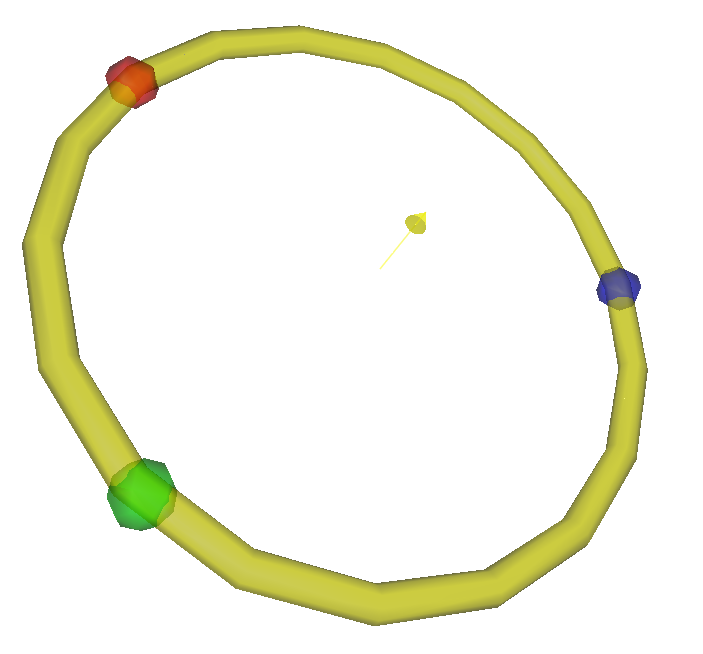
\includegraphics[scale=0.3]{DirectCircleFigure}
\caption{A circle (2-dimensional hyper-sphere) fit to three points.}
\end{figure}

Observe that the conformal model not only easily and
naturally solves the problem of fitting an $m$-dimensional hyper-sphere
to a set of $m+1$ points, but it also allows us to think of the blade directly
representative of that sphere in terms of any appropriate factorization
of vectors representative of points on that sphere.  We
can choose any $m+1$ points on the sphere to be in the outer product, provided they uniquely
determine the sphere.  We'll see examples of how this idea is
useful when we later solve certain problems using the conformal model.

Of course, not all sets of $m+1$ points determine
an $m$-dimensional hyper-sphere.  In the cases where these points don't determine a sphere, what do
we get?  To answer this question, we need to start with another definition.
%Well, we already know that if the $m+1$ points are co-$(m-1)$-hyper-spherical,
%then the outer product of the vectors directly representative of those points must be zero.
\begin{definition}\label{def_co_hyper_spherical}
For all $m\geq 0$, we say that the $m+2$ points $\{x_k\}_{k=1}^{m+2}\subset\V^n$
are co-$m$-hyper-spherical under the following circumstances.
\begin{equation*}
\begin{array}{l}
\mbox{For $m=0$, the points are identical.} \\
\mbox{For $m=1$, the points are co-point-pair.} \\
\mbox{For $m=2$, the points are co-circular.} \\
\mbox{For $m=3$, the points are co-spherical.} \\
\mbox{For $m=4$, the points are co-hyper-spherical.} \\
\mbox{etc.}
\end{array}
\end{equation*}
Here, $m$ corresponds to the dimension of the non-degenerate round upon
which all $m+2$ points lie.
\end{definition}

For the case $m=1$, if 3 points are non-co-point-pair, (which is to say that
they are non-co-$m$-hyper-spherical), then no two of those points are identical.
That is, they are pair-wise distinct.

With definition $\eqref{def_co_hyper_spherical}$ in place, consider $B\in\G$ as a blade directly representative
of an $m$-dimensional flat, where $m>0$.  Now convince yourself that $m+2$ points can
be found on the surface of this flat that are non-co-$(m-1)$-hyper-planar
and non-co-$m$-hyper-spherical.  By the first of these two conditions,
we know that there exists a subset of size $m+1$ of the $m+2$ points that
determines an $m$-dimensional hyper-sphere in the $m$-dimensional hyper-plane.
The second of these two conditions insures that the outer product
of the blade directly representative of this $m$-dimensional round
with the vector representative of the remaining point of the $m+2$
points is non-zero.  It follows that the vectors representative
of the $m+2$ points form a linearly independent set.  Then since
these points are on the hyper-plane, all that remains to be shown
to see that the outer product of the vectors representative of these
points is a scalar multiple of $B$ is to show that the grade of $B$ is $m+2$.
Knowing that the flat in question here is $m$-dimensional, we see that $B^*$
is of grade $n-m$ by result $\eqref{rslt_intersect_grades}$.
The grade of $B$ is therefore $n+2-(n-m)=m+2$.

For the case $m=0$, the case of flat-points, this argument doesn't work since clearly
one cannot find two unique points on a point.  Fortunately, a bit of work will show
that a flat point is directly represented by a 2-blade of the form $B=\lambda(i+xi\wedge\nvai)I$,
which simplifies to $B=-\lambda(\nvao\wedge\nvai+x\wedge\nvai)$.  (Here, $i$ is
the unit pseudo-scalar of the geometric algebra generated by $V^n$ and $I=i\wedge\nvao\wedge\nvai$ is
the unit pseudo-scalar of $\G$.)  It follows that
$\nvai\in B$.  Then since we can clearly find a vector representative of a point
that is on the flat-point, we see that $B$ factors as a scalar multiple of the outer
product of this vector and $\nvai$.  (Note that no vector representative of a point
is a scalar multiple of $\nvai$.)
\begin{figure}[H]
\centering
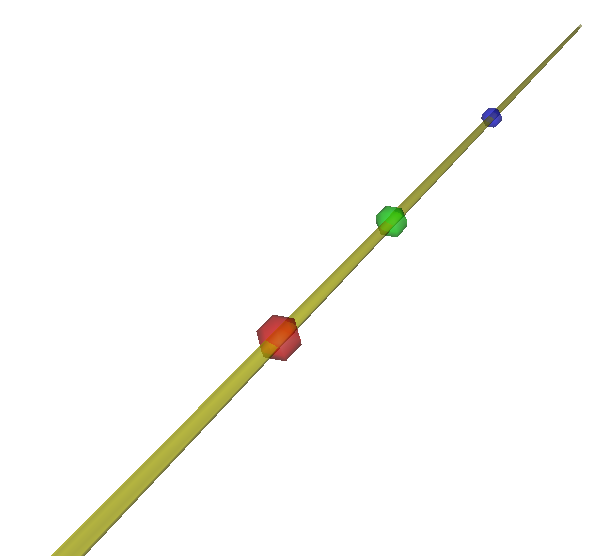
\includegraphics[scale=0.3]{DirectLineFigure}
\caption{A line (1-dimensional hyper-plane) fit to three points.}
\end{figure}
Interestingly, what we've learned so far is that all geometries,
with the exception of flat points, can be written as outer products
of vectors representative of points.  Our next result, however, will
show that we can represent direct flat geometries in what might be
considered a more convenient way.
\begin{theorem}\label{thm_round_to_flat}
If a blade $B\in\G$ directly represents a non-degenerate $m$-dimensional round,
then $B\wedge\nvai$ directly represents the $m$-dimensional flat
containing this $m$-dimensional round.
\end{theorem}
\begin{proof}
Let $\{x_k\}_{k=1}^{m+1}\subset\V^n$ be a set of $m+1$ points
such that $B=\bigwedge_{k=1}^{m+1} p(x_k)$.
Let $x_{m+2}\in\V^n$ be a point such that $p(x_{m+2})\wedge B\wedge\nvai=0$.
Then if $x_{m+2}$ is not on the round directly represented by $B$, it follows
that $p(x_{m+2})\wedge B\neq 0$, and therefore
\begin{equation*}
\nvai = \sum_{k=1}^{m+2}\alpha_k p(x_k),
\end{equation*}
where the scalars in $\{\alpha_k\}_{k=1}^m\subset\R$ are not all zero.
Our theorem now follows directly from lemma $\eqref{lma_lin_combo_points_is_inf}$.
\end{proof}

\section{Solving for Geometry}

Knowing how geometries of the conformal model factor in terms of vectors
representative of points leads us to one of the reasons why the conformal model
is a powerful analytical tool in geometry.  Specifically, if we're given two blades $A,B\in\G$ that
we know are both directly representative of the same non-single-point geometry, then we can easily show
that $A$ is a scalar multiple of $B$.  Let us state this formally with a theorem.
\begin{theorem}\label{thm_same_geos}
For any two blades $A,B\in\G$, if $G(A)=G(B)$ and these are not singletons,
then there exists a scalar $\lambda\in\R$ such that $A=\lambda B$.
\end{theorem}
\begin{proof}
With the exception of points and flat-points,
if $A$ and $B$ both directly represent the same geometry,
then any factorization of $A$ in terms of vectors representative of points will
also be, up to scale, a factorization of $B$.
\end{proof}
This is a powerful result, because the formulation
of $A$ may have been made one way, while the formulation of $B$, another, and now
we have found a way to relate the two formulations.  For example,
we might formulate $A$ as the intersection between two spheres.  Our result then tells us
that we can interpret $A$ as we would write the geometry represented by $A$ in a
canonical form $B$.  After composing $A$, we can decompose it as we would $B$.
The canonical form of $B$, in our example here, might be the intersection of a sphere centered on a plane.
Indeed, this is how the following figure was generated on a computer.
\begin{figure}[H]
\centering
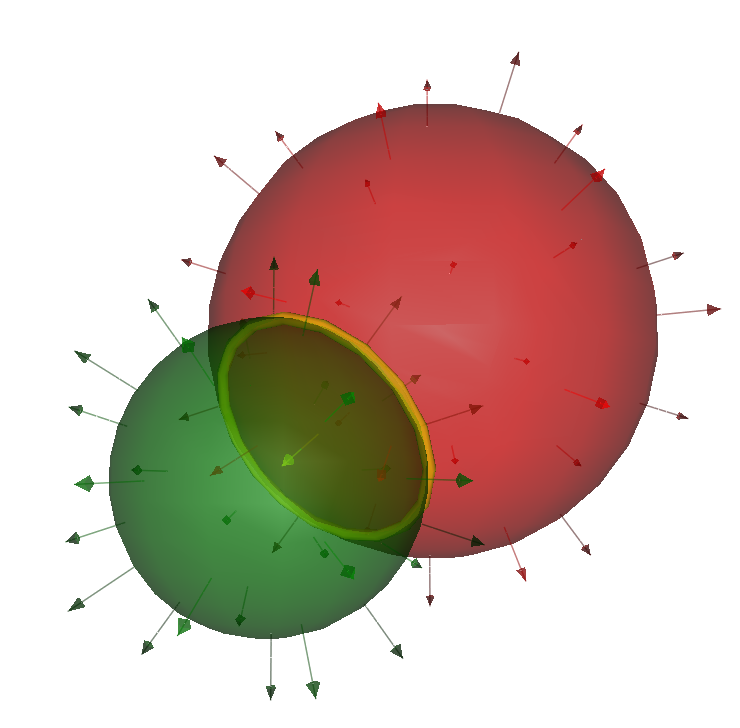
\includegraphics[scale=0.3]{RealIntersectionOfTwoSpheresFigure}
\caption{The intersection of two intersecting spheres.}
\end{figure}
Fascinatingly, the intersection of two non-intersecting spheres still gives us a
meaningful result in the conformal model.  What we get is an imaginary circle,
which we can draw just the same.
\begin{figure}[H]
\centering
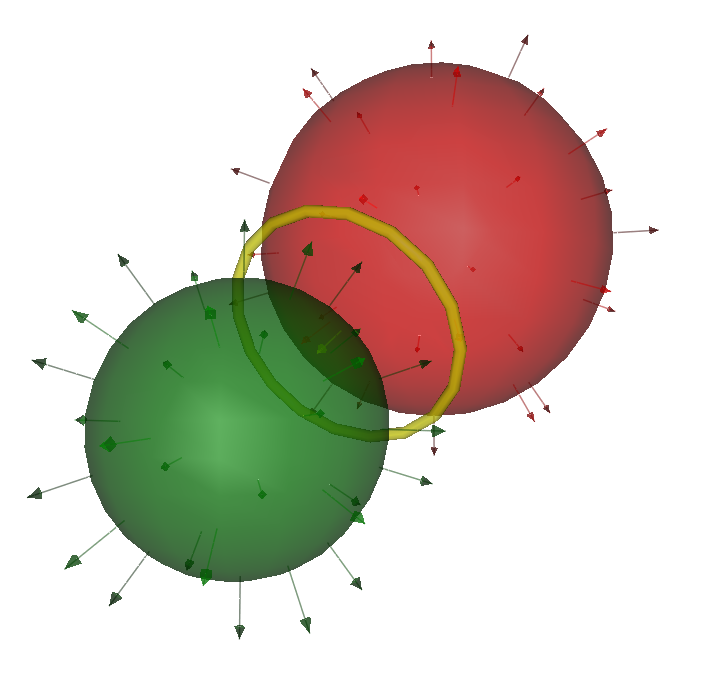
\includegraphics[scale=0.3]{ImaginaryIntersectionOfTwoSpheresFigure}
\caption{The intersection of two non-intersecting spheres.}
\end{figure}

Right away we can use theorem $\eqref{thm_same_geos}$ to come up with an important result.
\begin{theorem}\label{thm_flat_xor_round}
A blade $B\in\G$ directly represents a flat geometry if and only if
$B\wedge\nvai=0$.
\end{theorem}
\begin{proof}
By theorem $\eqref{thm_round_to_flat}$, the only reason we have to believe that $B\wedge\nvai\neq 0$
is in the case that $B$ is written entirely as the outer product of vectors representative of points.  But by theorem
$\eqref{thm_same_geos}$, we know that any such factorization of $B$ can
be rewritten as the outer product of a blade directly representative of a round
and $\nvai$.
\end{proof}
Notice that this theorem can also be stated as follows.  A blade $B\in\G$
directly represents a round geometry if and only if $B\wedge\nvai\neq 0$.
This is because every geometry is either round or flat.

Another useful feature of the conformal model comes from the way it lets
us think about doing operations at a high level.  We needed only descend to
the lower levels of thinking to develop the model.  Once developed, what we can do now is illustrated
by the following example.  Suppose we're given a dual circle $A$ and
a point $B$, and we want to find the dual sphere $C$ fitting these two geometries.
Well, we can think of $A^*$ as any three points determining the circle.
Combining this in the outer product with $C$, we then see that we
get what may be four points that determine the desired sphere.
Finally, we can come to the conclusion that $C=(A^*\wedge B)^*=A\cdot B$,
which is a nice result!  Our answer is simply the inner product of the two blades
representing the geometries in question.  Furthermore, the blade $C$ gives
us useful information in all situations.  If $C=0$, then $B$ was on $A$.
If $C\cdot\nvai=0$, then the sphere is really a plane and we may
think of it as a sphere centered at infinity with radius infinity.  In the remaining case, $C$ is
a finite sphere.

\section{Transforming Geometry}

Here we study the transformations of conformal geometries
by versors.  Let us therefore give a formal definition of such
elements.
\begin{definition}
Given any set of $m$ invertible vectors $\{v_k\}_{k=1}^m\subset\G(\V)$,
the element
\begin{equation*}
V = \prod_{k=1}^m v_k
\end{equation*}
is called a versor.
If $m$ is odd, we call $V$ an odd versor; if even, an even versor.
I will refer to $m$ as the grade of the versor $V$.
\end{definition}
It follows that versors are invertible by definition.  Clearly $V^{-1}=\tilde{V}/|V|$,
where $|V|=\prod_{k=1}^m |v_k|$.  It is also easy to see that versors
form their own group under the geometric product.  With versors as representative
of transformations, this property allows us to easily concatenate transformations.
As we'll come to find out, we can represent any conformal transformation with
a versor.  This is where the conformal model gets its name.

We will now proceed to lay some ground work
for a very import result that will help us decipher the action of versors on elements
representative of conformal geometries.

\begin{lemma}\label{lma_vector_invariance}
For any vector $a\in\V$, we have $VaV^{-1}\in\V$.
\end{lemma}
\begin{proof}
Notice that we need only show that for any vector $v\in\V$, we have $vav^{-1}=vav/|v|\in\V$.
By the equation
\begin{equation*}
vav = v(a\cdot v + a\wedge v) = (a\cdot v)v + v\cdot(a\wedge v)  = 2(a\cdot v)v - |v|^2a,
\end{equation*}
clearly this is the case.
\end{proof}
\begin{lemma}\label{lma_inner_prod_preserve}
Given any two vectors $a,b\in\V$, we have $VaV^{-1}\cdot VbV^{-1}=a\cdot b$.
\end{lemma}
\begin{proof}
It suffices to show that $\langle V(a\wedge b)V^{-1}\rangle_0=0$, since
\begin{equation*}
VaV^{-1}\cdot VbV^{-1} = \langle VabV^{-1}\rangle_0 = a\cdot b + \langle V(a\wedge b)V^{-1}\rangle_0.
\end{equation*}
A proof by induction is given.  Consider first $\langle v(a\wedge b)v^{-1}\rangle_0$, where $v\in\V$.
By direct evaluation, we get
\begin{equation*}
\langle v(a\wedge b)v^{-1}\rangle_0 = \frac{1}{|v|}
\left|\begin{array}{cc} n\cdot a & n\cdot a\\ n\cdot b & n\cdot b\end{array}\right| = 0.
\end{equation*}
Suppose now that for a fixed integer $k$, the versor $V$
of grade $k$ satisfies the lemma.  We must show that $\langle vV(a\wedge b)V^{-1}v^{-1}\rangle_0$ is zero.
To that end, it is not hard to see that
\begin{equation*}
\langle vV(a\wedge b)V^{-1}v^{-1}\rangle_0 =
\langle v\langle V(a\wedge b)V^{-1}\rangle_0 v^{-1}\rangle_0 +
\langle v\langle V(a\wedge b)V^{-1}\rangle_2 v^{-1}\rangle_0.
\end{equation*}
Clearly $\langle v\langle V(a\wedge b)V^{-1}\rangle_0 v^{-1}\rangle_0$ is zero by our inductive hypothesis.
That $\langle v\langle V(a\wedge b)V^{-1}\rangle_2 v^{-1}\rangle_0$ is zero follows directly from
the work we did to show that $\langle v(a\wedge b)v^{-1}\rangle_0$ is zero.
\end{proof}
We're now ready to prove a theorem that we'll use to prove something very interesting
about versor transformations in the conformal model.
\begin{theorem}\label{thm_outer_prod_preserve}
Given any $m$-blade $B=\bigwedge_{k=1}^m b_k$, we have
\begin{equation*}
VBV^{-1} = \bigwedge_{k=1}^m Vb_iV^{-1}.
\end{equation*}
\end{theorem}
\begin{proof}
Our proof of this theorem will rely upon the following.  If we find that $B=f(b_1,\dots,b_m)$,
where $f$ is any expression in the vector variables $b_1$ through $b_m$, then
clearly
\begin{equation*}
f(Vb_1V^{-1},\dots,Vb_mV^{-1})=\bigwedge_{k=1}^m Vb_iV^{-1}
\end{equation*}
by lemma $\eqref{lma_vector_invariance}$.
All that would remain, then, is to show that
\begin{equation*}
VBV^{-1}=f(Vb_1V^{-1},\dots,Vb_mV^{-1}),
\end{equation*}
and the theorem goes through.

We proceed now by strong induction.  Clearly the theorem holds for the case $m=1$.
The case $m=2$ is not much harder to prove.
Suppose now that for a fixed integer $m>2$, that the theorem holds for each case less
than $m$.  A partial expansion of $VBV^{-1}$ gives us
\begin{equation*}
VBV^{-1} = V(b_1\wedge\dots\wedge b_{k-1})b_kV^{-1} - (-1)^{k-1}V(a_k\cdot a_1\wedge\dots\wedge a_{k-1})V^{-1}.
\end{equation*}
We will consider each part of the right-hand side separately.  For the first part, we have
\begin{align*}
V(b_1\wedge\dots\wedge b_{k-1})b_kV^{-1} &=
V(b_1\wedge\dots\wedge b_{i-1})V^{-1}Vb_kV^{-1} \\
&= \left(\bigwedge_{i=1}^{k-1}Vb_iV^{-1}\right)Vb_kV^{-1},
\end{align*}
by our inductive hypothesis.  For the second part, we have
\begin{align*}
 & (-1)^k V(a_k\cdot a_1\wedge\dots\wedge a_{k-1})V^{-1} \\
 =& -(-1)^k V\left(\sum_{i=1}^{k-1}(-1)^i (a_k\cdot a_i)\bigwedge_{j=1,j\neq i}^{k-1} a_j\right)V^{-1} \\
 =& -(-1)^k\sum_{i=1}^{k-1}(-1)^i (a_k\cdot a_i)V\left(\bigwedge_{j=1,j\neq i}^{k-1} a_j \right)V^{-1} \\
 =& -(-1)^k\sum_{i=1}^{k-1}(-1)^i(Va_kV^{-1}\cdot Va_kV^{-1})\bigwedge_{j=1,j\neq i}^{k-1} Va_jV^{-1},
\end{align*}
by lemma $\eqref{lma_inner_prod_preserve}$ and our inductive hypothesis.
Having now sandwiched all vectors between $V$ and $V^{-1}$, our proof by
induction is complete.
\end{proof}
What theorem $\eqref{thm_outer_prod_preserve}$ tells us is that the function
$f(B)=VBV^{-1}$ is an outermorphism.  Applying this theorem, we get the following
important result.
\begin{result}\label{rslt_versor_action_on_geos}
Given a versor $V$, if we understand the transformation $Vp(x)V^{-1}$ for
any point $x\in\V^n$, then we understand the transformation $VBV^{-1}$,
where $B$ is any blade directly or dually representative of any geometry, with
the only exception being that of flat points.
\end{result}
\begin{proof}
In the previous section we showed that, with the exception of flat points,
all geometries directly represented by a blade $B$ may be written
as the outer product of vectors representative of points.  For all of
these geometries, our result goes through directly by theorem $\eqref{thm_outer_prod_preserve}$.

To show now that the theorem goes through for blades dually representative of geometries, (with again,
the exception of flat-points),
we need only show the commutativity of grade $k$ versors with the unit-psuedo scalar $I$ of $\G$.
For any vector $v\in\V$, it is not hard to show that $vI=(-1)^nIv$.  It follows that $VI=(-1)^{nk}IV$.
We then see that
\begin{equation*}
VBV^{-1} = -VBV^{-1}I^2 = -(-1)^{nk}VBIV^{-1}I,
\end{equation*}
which relates what we already know about the action of versors on blades directly
representative of geometries with those dually representative of such geometries.
\end{proof}
This is a fantastic result!  We now not only have a way of formulating a desired
transformation, but we also know that such a formulation, once formulated, will
apply to almost all geometries in the conformal model, no matter the representation!
This is similar to what we know about linear transformations.  A linear transformation
is entirely determined by how it transforms a basis of the space.  Therefore, if we
know how a desired transformation transforms a basis of the space, then we have
found the desired linear transformation.  Analogously, if we know how a desired
conformal transformation transforms a point, then we have found the desired
conformal transformation.  On the other hand, if we know how a given versor
transforms a point, then we can predict how it will transform any conformal
geometry, except flat points.

Flat points are an exception to the idea presented in result $\eqref{rslt_versor_action_on_geos}$,
because a given versor may not always leave $\nvai$ invariant up to scale.
We'll see an example of this in section $\eqref{sec_spherical_reflections}$ below.

We proceed now to develop the versor transformations of the conformal model.

\subsection{Reflections}\label{sec_reflections}

Interestingly, what we find in the conformal model is that a vector
not only represents a piece of geometry, but, as a versor, also represents
a transformation involving that geometry.  Specifically, a plane represents
a reflection about that plane, and a sphere represents a reflection about that
sphere!

Reflections turn out to be a very fundamental type of transformation, because
so many other types of transformations, such as rotations and translations, can be described
in terms of reflections about well chosen geometries.  For example, two
successive reflections about two well chosen planes gives us either a rotation
or a translation.  (Interestingly, this shows that the rotation and translation
transformations are perhaps not as dissimilar as we might have first thought them to be!)

Another type of reflection is performed about a sphere.  That is, a point
interior to a sphere is reflected out of it, while points exterior to the sphere
are reflected into it.  The question then comes up: if two successive
reflections about two well chosen planes gives us the rotation or
translation transformations, what does two successive reflections about
two well chosen spheres give us?  We will try to get to the bottom of this question soon enough.

Before we begin, however, it is worth mentioning a useful technique that we may
on occasion employ in the study of versor transformations.  Noting again that each vector
composing a given versor represents a piece of geometry, if they all share
a common point of interest, (sometimes a common center), then there is no loss
in generality when we restrict our attention to the case when this common point
is the origin, and this often simplifies calculations and derivations.
The reason is, (as we'll find out in section $\eqref{sec_translation_versors}$),
that there exists a translation versor $T\in\G$ such that if the versor $V\in\G$ in question
is given by
\begin{equation*}
V = \prod_{k=1}^m v_k,
\end{equation*}
for the $m$ vectors in $\{v_k\}_{k=1}^m$, then this transformation can be translated
to occur anywhere we want by
\begin{equation*}
TVT^{-1} = \prod_{k=1}^m Tv_kT^{-1}.
\end{equation*}
Remember, each vector $v_k$ composing the transformation versor $V$ represents a geometry
that we are free to act upon by any other transformation versor.

\subsection{Planar Reflections}\label{sec_planar_reflections}

Given a plane centered at $c\in\V^n$ with unit-length normal $v\in\V^n$,
here we consider the action of the vector dually representative of this plane
as a versor on a vector representative of a point.  That is, for $\pi=v+(v\cdot c)\nvai$,
what do we get in the evaluation of $\pi p(x)\pi^{-1}$?  Expanding this out, we get
\begin{equation*}
\pi p(x)\pi^{-1} = -p(y),
\end{equation*}
where $y=x-2(v\cdot (x-c))v$.  Drawing a picture
of this will convince you that $y$ is the reflection of $x$ about the plane!

Interestingly, here we have an example of a versor that leaves $\nvai$
invariant but for a factor of $-1$.  It follows that
\begin{equation*}
\pi(p(x)\wedge\nvai)\pi^{-1} = p(y)\wedge\nvai,
\end{equation*}
showing that flat points reflect about planes the same way round points do.

Having covered the case of flat points, we can now apply result $\eqref{rslt_versor_action_on_geos}$
to find that the versor $\pi$ reflects any conformal geometry about the plane represented by
$\pi$ as we would imagine.  Even a sphere partially straddling the plane will reflect as we would predict.
The following figure illustrates the reflection of a circle about a plane.
\begin{figure}[H]
\centering
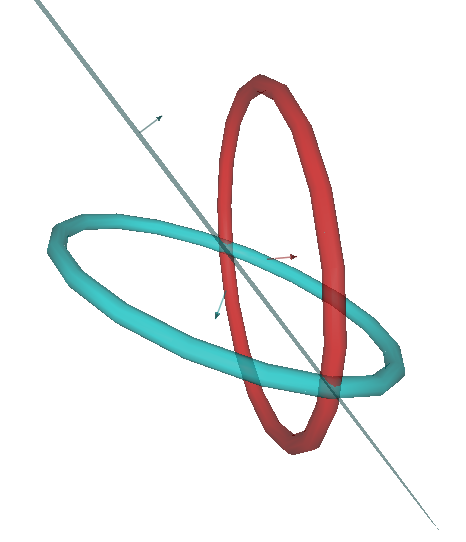
\includegraphics[scale=0.3]{ReflectionOfCircleAboutPlaneFigure}
\caption{The reflection of a circle about a plane.  The plane is shown here on edge.}
\end{figure}

\subsection{Translations}\label{sec_translation_versors}

It is not hard to imagine that we can perform a translation
using a single planar reflection about a well chosen plane.
The problem with this is that we need a different plane for
every situation involving a different point, even if the translation
vector is the same.  Interestingly, however, what we'll find is that
if we perform two successive reflections about two parallel planes, then
the positions of these planes becomes arbitrary, while only the relative
distance between the planes determines the amount of translation.
The direction of translation is determined by the attitude of the parallel planes.
It only takes a little bit of brain power to convince yourself that a point is consistently
translated by the two successive planar reflections in all three cases of where
a point can lie with respect to the two planes.

Let $v\in\V^n$ be a unit-normal shared by two parallel planes, let
$c\in\V^n$ be the position of the first plane, and $t\in\V^n$
be a vector representative of the desired amount of translation.
We assume that $v\wedge t=0$.
The versor $T$ representative of the translation is then given by
\begin{equation*}
T = (v+(v\cdot\left(c+\frac{1}{2}t\right)\nvai))(v+(v\cdot c)\nvai) = 1 - \frac{1}{2}t\nvai.
\end{equation*}
Notice that our result here is independent of the position of the
first plane, but only dependent upon the relative positions of
the two planes.
Of course, also notice that $v$ goes away as $t$ is all that
is needed to characterize the translation transformation.

% Give polar decomposition?

\subsection{Rotations}

Suppose now that the two planes we reflect about are
non-parallel.  In this case we get a rotation.  Let $c\in\V^n$
be a common point among the two planes, and let $v_0,v_1\in\V^n$
be their unit-normals, respectively.  Not being parallel planes,
we have $v_0\wedge v_1\neq 0$.  We can then let $a\in\V^n$
be a unit-length vector representing the axis of rotation, and
let $\theta\in\R$ be the angle of rotation.  Doing so, we see
that $v_0\wedge v_1=-ai\sin\theta/2$.  The versor that
represents a rotation about the point $c$ is then given by
\begin{equation*}
(v_0+(v_0\cdot c)\nvai)(v_1+(v_1\cdot c)\nvai) = \cos\frac{\theta}{2} - (a+a\wedge c\wedge\nvai)i\sin\frac{\theta}{2}.
\end{equation*}
Letting $c=0$, we get the well-known rotor in Euclidean geometric algebras which
has a polar decomposition of $\exp(-ai\theta/2)$.

\subsection{Spherical Reflections}\label{sec_spherical_reflections}

Let $c\in\V^n$ be the center of a sphere, and $a\in\V^n$ be a point
exterior to the sphere.  Then the point $b\in\V^n$ along the line
from $c$ to $a$ given in the following figure is what we refer to
as the reflection of $a$ in the sphere.\footnote{The vector $a$ is
also what we may refer to as the the reflection of $b$ in the sphere or about the sphere.}
\begin{figure}[H]\label{fig_spherical_reflection}
\centering
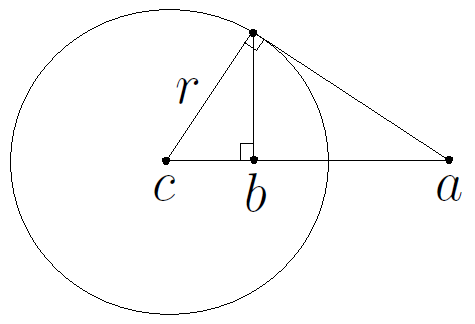
\includegraphics[scale=0.3]{SphericalReflectionFigure}
\caption{The reflection of a point about a sphere.}
\end{figure}
We let $r\in\R$ be the radius of this sphere.  Using what we know about similar
triangles, it is not hard to show that $b = (1-\lambda)c + \lambda a$,
where
\begin{equation*}
\lambda = \left(\frac{r}{|c-a|}\right)^2 = \left(\frac{|c-b|}{r}\right)^2,
\end{equation*}
the square of a common ratio between respective sides of the
similar triangles in the figure above.
Interestingly, letting $\sigma=p(c)-\frac{1}{2}r^2\nvai$ represent the sphere in the figure, we find that
\begin{equation*}
\sigma p(a)\sigma^{-1} = -\lambda^{-1}p(b),
\end{equation*}
showing that vectors dually
representative of spheres perform, as versors in a versor transformation, spherical reflections!
As one would expect, a double spherical reflection about the same sphere leaves a point
invariant.  This is because we also find that
\begin{equation*}
\sigma p(b)\sigma^{-1} = -\lambda p(a).
\end{equation*}

Applying result $\eqref{rslt_versor_action_on_geos}$, we find that $\sigma$, when
acting upon a blade directly representative of a line, gives us the blade directly
representative of the circle that is the reflection of that line in the sphere.
The following figure illustrates this.
\begin{figure}[H]
\centering
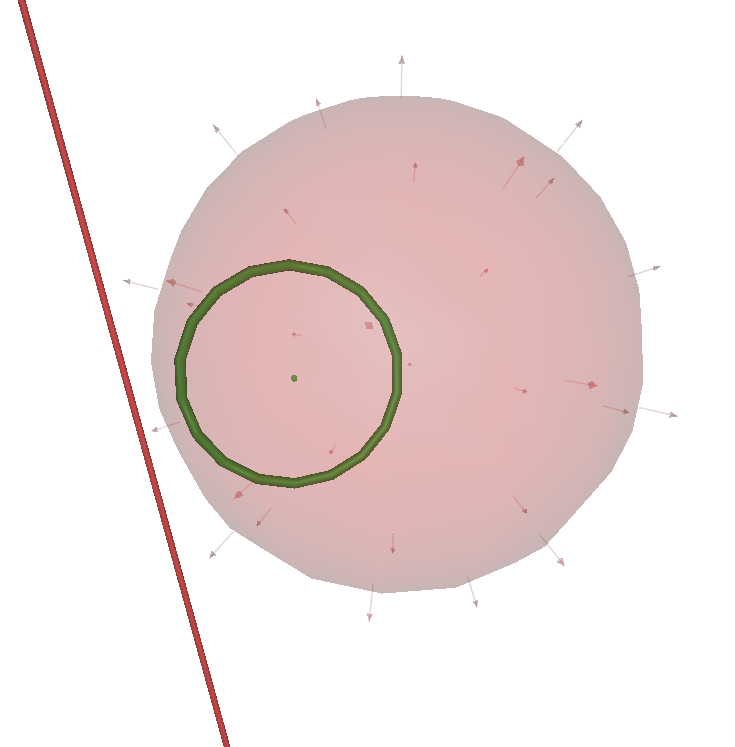
\includegraphics[scale=0.3]{ReflectionOfLineInSphereFigure}
\caption{The reflection of a line in a sphere.}
\label{fig_sph_ref_of_line}
\end{figure}
Similarly, the reflection of a plane in a sphere is a sphere.

Of course, result $\eqref{rslt_versor_action_on_geos}$ doesn't tell us anything about
how $\sigma$ acts on a flat point.  The key, as always, is to see how the versor, (in this case $\sigma$), acts on $\nvai$.
Investigating this, we find that
\begin{equation*}
\sigma(p(a)\wedge\nvai)\sigma^{-1} = \frac{2}{(c-a)^2}p(b)\wedge p(c),
\end{equation*}
showing that $\sigma$ transforms the flat point at $a$ into the pair of points $b$ and $c$.
This is because the spherical reflection of a sphere's center is, up to scale, $\nvai$ and vice-versa.
Specifically, we have
\begin{equation*}
\mbox{$\sigma p(c)\sigma^{-1}=-\frac{1}{2}r^2\nvai$ and $\sigma\nvai\sigma^{-1}=\frac{-2}{r^2}p(c)$.}
\end{equation*}

It is important to notice here that spherical reflections, unlike planar reflections, do
not generally preserve geometric type.  As we saw in figure \ref{fig_sph_ref_of_line},
the spherical reflection of a line became a circle, a different type of geometry than
what we started with.  Indeed, as we just saw, the spherical reflection of a sphere's
center in itself is a multiple of $\nvai$ which, by definition, both dually and directly represents
the empty point-set geometry or the geometry of nothing.\footnote{Some authors refer to $\nvai$ as the point at
infinity.  This idea may come from observing the point $\sigma p(x)\sigma^{-1}$ as $x$
approaches $c$.  But as the direction from which $x$ approaches $c$ is significant to me,
and ideas like a point at infinity seem too ill-defined and poorly addressed, I prefer to think of $\nvai$
as I have just described it.  It is important to realize that the language of some proofs given in this
paper depend upon the fact that $\nvai$ is, by definition, not representative of a point in $\V^n$.}
The non-preservation of geometric type means that we'll need
to take greater care in deciphering transformations involving spherical reflections.

So far we have only considered the spherical reflections of flat geometries, and it is
not too hard to see that these are always round.  Interestingly, however, the reverse
is not generally true.  That is, the spherical reflection of a round geometry is not
always flat.  To see this, first consider the reflection of any sphere in a sphere.
This is always a plane.  Now consider any circle sharing all points with a sphere to be
spherically reflected and realize that the spherical reflection of this circle must be
contained within the plane that is the spherical reflection of that sphere.  What we find is
that circles, under most circumstances, spherically reflect as circles, and only
under a certain condition, spherically reflect as lines.  Specifically, the center
of the sphere to be reflected about must be in the plane determined by the
circle for the circle to be spherically reflected as a line.

Lastly, before moving on, we should not forget to
consider the spherical reflection of a point in a degenerate sphere.  This
type of reflection simply can't be taken, because in this case $\sigma^{-1}$ does not exist.

\subsection{Dilations}

Dilations occur as two successive spherical reflections about two concentric
spheres of differing volume.  The best analogy for this, I believe, is that of what we did to formulate
translations as two success planar reflections about two distinct and parallel planes.
As with that case, here, when we consider the three cases of where a point can lie
with respect to the three partitions of space created by the two spheres, we can convince ourselves
that the double spherical reflections consistently produce a dilation in each case.

Here we will take the approach mentioned in section $\eqref{sec_reflections}$,
and restrict our attention, without loss of generality, to dilations that occur at the
origin.  The two spheres dually represented by $\sigma_0$ and $\sigma_1$, therefore,
will be placed at the origin, and we will give them $r_0,r_1\in\R$ as their respective radii.
We then find that
\begin{equation}\label{equ_dilation}
r_0^{-4}\sigma_1\sigma_0 p(x)\sigma_0\sigma_1 = p\left(\frac{r_1^2}{r_0^2}x\right),
\end{equation}
which makes it very clear what the action of the versor $\sigma_1\sigma_0$ does
to any conformal geometry!\footnote{The verification of equation $\eqref{equ_dilation}$
by hand proved to be too error-prone for me, so here I resorted to the use of a computer
algebra system.  Such systems often prove quite useful in the exploration of geometric algebras.}
We can also see how the dilation changes when
we consider the two cases $r_0<r_1$ and $r_0>r_1$.  Dilations may therefore
push things away or pull them closer.

\subsection{Transversions}

% points of invariance help out.

Transversions are the strange duck in the family of fundamental
transformation versors of the conformal model.  A transversion is two
successive reflections about two spheres of the same radius that share a single point
of contact.  (By having the same radius, notice that we cannot let one sphere
envelop the other.)
Letting $V=\sigma_1\sigma_0$, where $\sigma_0=\nvao+c$
and $\sigma_1=\nvao-c$, $c\in\V^n$ being the center of one of the two spheres
with $-c$ being the center of the other sphere, we get
\begin{equation*}
\frac{Vp(x)\tilde{V}}{c^4(1+4\frac{x^2}{c^2}-4\frac{c\cdot x}{c^2})}
= p\left(\frac{x-2\frac{x^2}{c^2}c}{1+4\frac{x^2}{c^2}-4\frac{c\cdot x}{c^2}}\right).
\end{equation*}
From this it may not be entirely clear how transversions act
on points, (it is certainly not obvious to me), and therefore it may be even less clear how such transformations
act on geometries of the conformal model.  For example, we can reason
that, under a transversion, a plane must transform into a plane.  It is
first spherically reflected into the sphere represented by $\sigma_0$
as a sphere, then spherical reflected into the sphere represented by $\sigma_1$
as a plane.  But can we visualize in all cases the spacial relationship between
the initial plane and the final plane?

Of course, a great technique for dealing with certain difficult problems is sometimes
to transform them into another equivalent problem.  For example, if a direct proof seems hard to find,
sometimes considering the contrapositive more easily leads to a proof.  In the case
of transversions, it can be shown that our description of a transversion is equivalent
to a different sequence of reflections.  Specifically, a transversion can also be described
as a spherical reflection, followed by a translation, followed by a spherical reflection
in the same sphere.  Notice that both reflection sequences have a single
point of invariance.  For the original transversion description, this point is the
point of contact between the two spheres.  For the new transversion description,
it is the center of the sphere in which we twice reflect.  Showing that the two
reflection sequences are equivalent, we'll therefore place a sphere represented
by the vector $\sigma$ at the origin.  Then, giving the sphere a radius of $|c|$,
and letting $T=1-c\wedge\nvai$ be the translation versor for the transversion, (notice that the translation
vector here is $2c$), we then find that
\begin{equation*}
\sigma T\sigma = -\sigma_1\sigma_0.
\end{equation*}
The difference in sign doesn't matter, since when the versor is used, it cancels itself
out.\footnote{Not that it is the case here, but even if one of the two transformations preserved
handedness while the other did not, we could still substitute one for the other as a replacement
in our study of the overall transformation.}

Does this bring us any closer to understanding transversions?  Well, while this alternative
construction of transversions may or may not be more intuitive, it makes sense to me
that an intermediate translation between two spherical reflections may be a useful idea.
Without the translation, the spherical reflections leave a geometry invariant.  Translating
the reflected geometry before it's reflected back out of the sphere may have its applications
in certain problems of geometry and may lead to some interesting results.

\subsection{Other Transformations}

Yet more types of transformations can be constructed in the conformal model
by combining the above mentioned transformations.  For example, general
rigid body motions can be formulated by combining the rotation and translation
versors.  Questions should be answered about the set of all possible types
of transformations, what groups they form under versor concatenation, what
their exponential forms are, and if their logarithms can be taken, but
this is beyond the scope of this paper and, admittedly, the present capabilities of the author.

In any case, it should be clear that by combining all types of reflection vector versors, (planar and spherical),
that we exhaust all possible transformations by versors that we can come up with in the
conformal model.\footnote{Notice that we didn't consider spherical reflections in an imaginary sphere.
We leave this too as outside the scope of the present paper.}
A more thorough treatment of versor transformations in the conformal model can be found in
\cite{dorst07}.
We have only begun to discover what types of transformations we
can do with these basic building blocks.  (There are undoubtedly many more combinations to
consider.)  But we will leave versor transformations for now, content with what we have
covered thus far as an introduction to the subject.

\section{Reflections Are Geometry}

In this section we prove that every blade representative of a conformal geometry
is also a versor representative of a reflection about that geometry.  The cases
of the $n$-dimensional hyper-sphere and the $(n-1)$-dimensional hyper-plane
have already been proven.  Knowing that any flat is an outer product
of blades dually representative of $(n-1)$-dimensional hyper-planes and
that any round is an outer product of a blade dually representative of an $n$-dimensional
hyper-sphere and a blade dually representative of a hyper-plane of the same
dimension as the round, we need only show here that such blades have factorizations
in terms of vectors that are pair-wise orthogonal.  We state this formally as a
result since we will call upon it in later sections.
\begin{result}\label{rslt_reflections_are_geometry}
Any blade $B\in\G$ directly or dually representative of a conformal geometry
is also a versor.  Furthermore, this versor represents a reflection about that geometry.
\end{result}
\begin{proof}
The case of flats is trivial.  Let $c\in\V^n$ be a point on a flat
characterized by the intersection of $m$ planes of dimension $n$.
Let $\{v_k\}_{k=1}^m\subset\V^n$ be the set of normal vectors for each of these planes.
It is clear that such a set can be found such that for all $i\neq j$, we have
$v_i\cdot v_j=0$.  Then for all $i\neq j$, we have $(v_i+(c\cdot v_i)\nvai)\cdot(v_j+(c\cdot v_j)\nvai)=0$.
It follows that a blade dually representative of this flat can be written
as a geomtric product of vectors.

The case of rounds is also trivial.  Let $c$ now be the center of the round
and $r$ be the radius of the round.  We can then form the round
as $(p(c)-\frac{1}{2}r^2\nvai)\cdot\pi$, where $\pi$ is a versor dually
representative of a flat.  Then for any $v\in\V^n$, if $(v+(c\cdot v)\nvai)$ is any vector
in the composition $\pi$, notice that
\begin{equation*}
\left(p(c)-\frac{1}{2}r^2\nvai\right)\cdot(v+(c\cdot v)\nvai)=c\cdot v-c\cdot v = 0.
\end{equation*}
We have now proven the result for all dual representatives.  To see that any direct
representative is also a versor, notice that the dual of any versor is a versor.  (I may
need to prove this.  Is it true?)
\end{proof}

\section{Inference Of Geometry}

Given a blade $B\in\G$, is it possible for us to infer what type of geometry it
represents, dually or directly?  Our first clue is the grade of $B$.
For example, we summarize what types of geometries can be represented by the various
grades in the conformal model of 3-dimensional space in the following table.
\begin{equation*}
\begin{array}{ccccc}
 &  & \mbox{Dual} & & \mbox{Direct} \\
\hline
1 & \vline & \mbox{Sphere, Plane, Point} & \vline & \mbox{Point} \\
2 & \vline & \mbox{Circle, Line} & \vline & \mbox{Point-Pair, Flat-Point} \\
3 & \vline & \mbox{Point-Pair, Flat-Point} & \vline & \mbox{Circle, Line} \\
4 & \vline & \mbox{Point} & \vline & \mbox{Sphere, Plane, Point}
\end{array}
\end{equation*}
Given a blade of any of these 4 grades, one could restrict their attention to
only the grades 1 and 2 by taking the dual of blades of grades 3 and 4.
In any case, we will not give a full and comprehensive treatment of
geometric inference here, but we will give an important result on this subject
which also puts focus on a type of geometry that, until now, we have
mentioned, but not given any significant attention.  
The type of geometry I speak of here is the imaginary kind.
Specifically, what is meant by this is any round represented by
a blade $B\in\G$ of the form
\begin{equation*}
B = \sigma\wedge A,
\end{equation*}
where the blade $A\in\G$ is dually representative of a hyper-plane containing
a point $c\in\V^n$, and $\sigma$ is given by
\begin{equation*}
\sigma = p(c) + \frac{1}{2}r^2\nvai,
\end{equation*}
where $r\in\R$ is non-zero.  Notice that $\sigma$ here does not dually
represent an $n$-dimensional hyper-sphere.  In fact, and strictly speaking,
like $\nvai$, it represents the empty-set geometry or the geometry of nothing.
That is, there is no point $x\in\V^n$ such that $p(x)\cdot\sigma = 0$.  We say
that $B$ is dually representative of an imaginary round.

We now give the promised result and go on to prove it.
\begin{result}
If $m<n$, then a blade $B\in\G$ directly representative of an $m$-dimensional real hyper-sphere
is also dually representative of an $(n-m)$-dimensional imaginary hyper-sphere.
\end{result}
\begin{proof}
Our first task is to show that two such types of geometry can be represented by
a blade of the same grade.  Given our description of imaginary rounds above,
it is not hard to see that result $\eqref{rslt_intersect_grades}$ also applies to imaginary rounds.
An imaginary $(n-m)$-dimensional round is therefore dually represented by a blade
of grade $n-(n-m)+1=m+1$.  Applying this result again, a real $m$-dimensional round
is directly represented by a blade of grade $n+2-(n-m+1)=m+1$.

We proceed now to give a proof by induction.  We start with the case $m=n-1$.
This case is proved by the following identity, which the reader can check.\footnote{
Multiply the left side of the identity by the unit translation versor $T=1+\frac{1}{2}c\wedge\nvai$ and the right
side by $\tilde{T}$.  This makes proving the identity easier.}
\begin{equation*}
2r(p(c)+\frac{1}{2}r^2\nvai)\wedge(v+(c\cdot v)\nvai) = p(c-rv)\wedge p(c+rv).
\end{equation*}
Here, $v\in\V^n$ is a unit-length vector.

For the inductive step, let $\sigma_i$ dually represent the imaginary round,
and let $\sigma_r$ directly represent the real round.  Then without loss of generality,
we may center each of these at the origin.  Now notice that for a given unit-length
vector $v\in\V^n$, we have $rv\wedge\sigma_i\neq 0$ if and only if $rv\wedge\sigma_r\neq 0$
since $\sigma_i$ is a scalar multiple of $\sigma_r$ which is our inductive hypothesis.
It is then easy to see that $r(v+(0\cdot v)\nvai)\wedge\sigma_i=rv\wedge\sigma_i$, if non-zero,
is dually representative of an imaginary sphere of one lower dimension.  Then, if
it can be shown that $rv\wedge\sigma_r=p(rv)\wedge\sigma_r$, then this blade is directly representative
of a real sphere of one higher dimension, and our proof is complete.  To that end,
write $\sigma_r$ as $(\sigma\wedge\pi)I$, where $\sigma$ is a vector dually representative
of an $n$-dimensional hyper-sphere centered at the origin with radius $r$, and
$\pi$ is a vector dually representative of a hyper-plane containing the origin.
So we have $p(0)\cdot\pi=\nvao\cdot\pi=0$.  Also notice that $\nvai\cdot\pi=0$
by theorem $\eqref{thm_flat_xor_round}$, and that $p(rv)\cdot\sigma=0=rv\cdot\sigma$, since
the point represented by $p(rv)$ is on the sphere represented by $\sigma$ which is at the origin.  We then have
\begin{align*}
p(rv)\wedge\sigma_r &= p(rv)\wedge(\sigma\wedge\pi)I \\
 &= (p(rv)\cdot(\sigma\wedge\pi))I \\
 &= ((p(rv)\cdot\sigma)\pi - (p(rv)\cdot\pi)\sigma)I \\
 &= ((rv\cdot\sigma)\pi - (rv\cdot\pi)\sigma)I \\
 &= rv\wedge\sigma_r.
\end{align*}
Of course, this induction must terminate, because there is no imaginary sphere
of zero dimension.
\end{proof}

\section{Non-Homogenized Geometry}

A vector $v\in\V$ dually representative of an $n$-dimensional hyper-sphere
is homogenized whenever $\nvai\cdot v=-1$, which implies that $v^2=r^2$.
(Note that the converse is not true.)
If $v\in\V$ is dually representative
of an $(n-1)$-dimensional hyper-plane, then $v$ is homogenized whenever
$\nvao\wedge\nvai\cdot v\wedge\nvai$ is a unit-length vector in $\V^n$,
which implies that $v^2=1$.  (In this case the converse does hold.)
Now since all rounds and flats can be constructed as outer products of
such vectors, we can, up to handedness, define a blade dually representative
of any geometry as being in a homogenized form when each vector in a given factorization
of that blade is homogenized.  The handedness of the blade will depend
on the order in which we take the vectors in the outer product and we
do not want our definition of a homogenized form to depend on such order.

The general question we're concerned with in this section is as follows.
If a given blade $B\in\G$ that is the result of some geometric operation is
not in a homogenized form, then what is the geometric significance of the scalar
$\lambda\in\R$ such that $\lambda^{-1}B$ is a homogenization of $B$?
As we have already seen in section $\eqref{sec_spherical_reflections}$,
spherical reflections in homogenized sphere representatives require homogenization
by a scalar that is also a ratio significant to the transformation.
We can even see that this transformation negates handedness in this case.
In section $\eqref{sec_planar_reflections}$, we saw that planar reflections
of flat points preserve handedness, but not the handedness of round points, but
other than all this, homogeneous forms are invariant under this type of transformation.

So the answer to this question depends upon the geometric operation.
Since we don't have time here to consider every possible geometric
operation of significance,\footnote{Notice that every geometric operation
of significance is simply every operation possible in $\G$.  Mathematics
cannot produce a meaningless result.}
here we will choose one that is fundamental
to the conformal model.
Given a blade $B\in\G$ dually representative
of some geometry, and a point $x\in\V^n$, we know that $p(x)\cdot B=0$
if and only if $x$ is a part of the geometry represented by $B$.  However,
when $p(x)\cdot B\neq 0$, what geometry does the resulting blade represent dually,
and how might we interpret the geometric significance of the scalar needed to
homogenize this blade?  No doubt, if $B\in\V$, the scalar $p(x)\cdot B$ will
have some sort of geometric significance itself.

Suppose first that $B$ dually represents an $m$-dimensional
hyper-plane with $m<n$.  It then follows by result $\eqref{rslt_intersect_grades}$
that there exists a set of $n-m$ vectors $\{\pi_k\}_{k=1}^{n-m}$
such that $B=\bigwedge_{k=1}^{n-m}\pi_k$, where for each integer
$k\in[1,n-m]$, $\pi_k$ is a homogenized vector representative
of an $n$-dimensional hyper-plane.  Then, without loss of generality,
we can assume that exactly $n-m-1$ of these vectors are representative
of a hyper-plane containing the point $x$.
It follows that for some integer $k\in[1,n-m]$, we have
\begin{equation*}
p(x)\cdot B = -(-1)^k (p(x)\cdot \pi_k)\bigwedge_{i=1,i\neq k}^{n-m} \pi_k.
\end{equation*}
We see now that the geometry being dually represented here is an
$(m+1)$-dimensional hyper-plane containing $x$ and
the hyper-plane represented by $B$.\footnote{Notice that this really isn't a new result.
Simply realize that $p(x)\cdot B = (p(x)\wedge BI)I$.}
%-- This may not be true, on second thought.
%  Furthermore, this shows that
%homogeneous forms are not unique for blades of grades greater than one, because $(p(x)\wedge BI)I$ is in homogeneous
%form while $p(x)\cdot B$ is in need of homogenization.  This blade therefore has more than one homogeneous form.}
This result also reveals the possible
change in handedness inherent in this type of geometric operation.  All that remains now is to determine
the geometric significance of the homogenization scalar $p(x)\cdot\pi_k$.
Letting $v\in\V^n$ be a unit-length vector
normal to the hyper-plane $\pi_k$, and letting $\alpha\in\R$ be a scalar such that
$x-\alpha v$ is a point on this hyper-plane, we find that
\begin{equation*}
p(x)\cdot\pi_k = p(x)\cdot(v+(v\cdot(x-\alpha v))\nvai) = \alpha.
\end{equation*}
Here, $|\alpha|$ is the shortest or orthogonal distance
of $x$ to the hyper-plane represented by $\pi_k$, which is also the shortest distance
from $x$ to the hyper-plane represented by $B$!

Suppose now that $B$ dually represents an $m$-dimensional
hyper-sphere with $m\neq n$.  We break the problem into
two cases.  In the first case, $x$ is in the $m$-dimensional
hyper-plane determined by $B$, and in the second case,
$x$ is not in this hyper-plane.  In the first case, let $\pi\in\V$
be a vector dually representative of this $m$-dimensional
hyper-plane such that $B=\sigma\wedge\pi$, where $\sigma\in\V$
dually represents an $n$-dimensional hyper-sphere with center $c\in\V^n$
and radius $r\in\R$.  It follows that
\begin{equation*}
p(x)\cdot B = (p(x)\cdot\sigma)\pi,
\end{equation*}
which is an interesting result, because now we have a hyper-plane instead of a hyper-sphere.
The homogenization scalar is then given by
\begin{equation}\label{equ_point_dot_sphere}
p(x)\cdot\sigma = \frac{1}{2}(r^2-(x-c)^2),
\end{equation}
which is somewhat analogous to our earlier result, but is not quite the shortest
distance between $x$ and the round represented by $B$.  This isn't too surprising,
since calculating such a distance is not so trivial anyway.

In the second case, we can invoke result $\eqref{rslt_intersect_grades}$ to
see that there must exist $n-m+1$ vectors $\{\sigma_k\}_{k=1}^{n-m+1}$
such that $B=\bigwedge_{k=1}^{n-m+1}\sigma_k$, where for each
integer $k\in[1,n-m+1]$, $\sigma_k$ is a homogenized vector representative
of an $n$-dimensional hyper-sphere.  Then, without loss of generality,
we can assume that exactly $n-m$ of these vectors are representative
of a hyper-sphere containing the point $x$.  It follows that for some integer $k\in[1,n-m+1]$,
we have
\begin{equation*}
p(x)\cdot B = -(-1)^k(p(x)\cdot\sigma_k)\bigwedge_{i=1,i\neq k}^{n-m+1}\sigma_k.
\end{equation*}
We see now that the geometry being dually represented here is an $(m+1)$-dimensional
hyper-sphere containing $x$ and the hyper-sphere represented by $B$.  Again,
this result reveals the possible change in handedness inherent in this type of geometric operation.
All that remains now is to determine the geometric significance of the homogenization
scalar $p(x)\cdot\sigma_k$.  Choosing a center $c$ and radius $r$ for the sphere
represented by $\sigma_k$, we get the result in equation $\eqref{equ_point_dot_sphere}$,
but notice that we have a slightly different context here.  Here, $c$ is not necessary
the center of the hyper-sphere represented by $B$.  The point $c$ is probably
almost anywhere along a line orthogonal to the $m$-dimensional hyper-plane
determined by $B$.

\section{More Geometry}

Rounds and flats are the extent of geometric primitives available in the conformal
model of geometric algebra.  If we, however, allow for a small variation in the way
geometries are represented in the conformal model, we open up a whole new set
of geometric primitives.

\begin{definition}
Let $g:\V^n\to\G$ be any blade-valued function of a point variable.
We then say that $g$ is directly representative of a geometry as
the set of all points
\begin{equation*}
G(g)=\{x\in\V^n|p(x)\in g(x)\}.
\end{equation*}
Similarly, we say that $g$ is dually representative of a geometry as the set
of all points
\begin{equation*}
G^*(g) = \{x\in\V^n|p(x)\in g^*(x)\}.
\end{equation*}
Here, $g^*(x)$ refers to either of the two functions $\pm g(x)I$.
We refer to $g$ as a geometric function.
\end{definition}
From this definition it is clear that all geometric primitives of the conformal model
are recovered by the set of all constant geometric functions.  Realizing that
all vectors representative of points are null, we see that $p$ is a geometric
function both dually and directly representative of the geometry that is all
of space $\V^n$.

One of the motivations behind geometric functions comes from a method
of derivation for the dual forms of the sphere and plane primitives of
the conformal model.  After writing a vector equation equated to zero,
one can see how $p(x)$ factors out of this equation in terms of the inner product.
However, for such vector equations whose solution sets are infinitely long cylinders,
right-circular conical surfaces or ellipsoids, the function $p(x)$ factors out of such
equations leaving a non-constant blade.  Embracing the result, we begin a
development of geometric functions.

Where we run into trouble with geometric functions, however, is in the
use of what was such a convenient tool for geometric analysis
in the original model.  Geometric functions that are
canonical forms, while easily lending themselves to the decomposition
of the represented geometry into its characteristic parts, cannot
be used to decipher the result of a geometric operation in the way
to which we were accustomed in the traditional model.
In other words, there is no direct equivalent
of theorem $\eqref{thm_same_geos}$ for geometric functions.
Indeed, for any two geometric functions $g_1$ and $g_2$, if $G(g_1)=G(g_2)$,
we cannot conclude that there exists a scalar $\lambda\in\R$ such that for all
$x\in\V^n$, we have $g_1(x)=\lambda g_2(x)$.
This may not mean, however, that canonical forms are no longer useful to us.
If we really can show, given two geometric functions $g_1$ and $g_2$,
that for all $x\in\V^n$, we have $p(x)\in g_1(x)$ if and only if $p(x)\in g_2(x)$,
and if one of these, say $g_1$, is in a canonical form, then we can use that form to decompose
the represented geometry into its characteristics parts, and then rightly attribute these
characteristics to the geometry represented by $g_2$ as well as $g_1$.

Admittedly, the idea of geometric functions is somewhat contrary to the vision most people have about
a geometric algebra.  The holy grail, so to speak, of a geometric algebra
is the idea that for any geometry we could think of, there exists an element
in the algebra representative of that geometry, and all possible geometric
operations are available and closed in the algebra.  Furthermore, any question
about a given geometry should be answerable through some kind of calculation
in the algebra.  Perhaps we need a better geometric algebra
and even a new type of model implemented in that algebra, but until then,
let's continue on.

Our first specimen is important to geometry.
It is the general conical surface as illustrated in the following figure.
\begin{figure}[H]
\centering
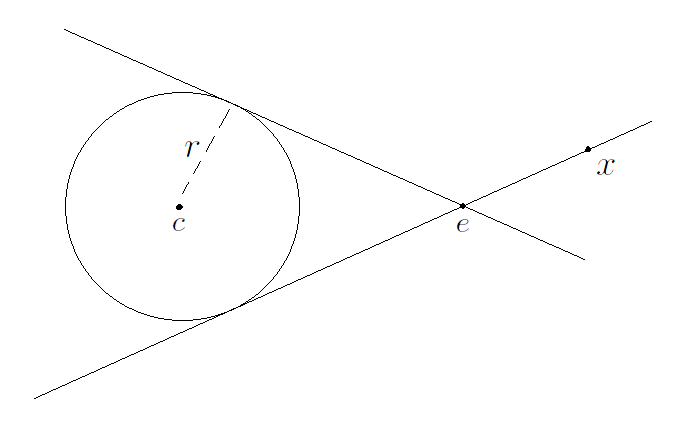
\includegraphics[scale=0.4]{GeneralConicalSurfaceFigure}
\caption{The general conical surface centered at a point $e$ and touching a sphere centered at $c$ with radius $r$.
The point $x$ is on the surface.}
\end{figure}

A geometric function dually representative of this surface is given by
\begin{equation*}
S(x) = p\left(\frac{c-s(x)e}{1-s(x)}\right)-\frac{1}{2}\left(\frac{r}{1-s(x)}\right)^2\nvai,
\end{equation*}
where $s(x)$ is defined as
\begin{equation*}
s(x) = \frac{(x-e)\cdot(x-c)}{(x-e)^2}.
\end{equation*}
Replacing $e$ with $e+\lambda v$, where $\lambda\in\R$ and $v\in\V^n$ is a unit-length vector,
we see that
\begin{equation}\label{equ_cylinder}
\lim_{\lambda\to\infty} S(x) = p(c+[(x-c)\cdot v]v)-\frac{1}{2}r^2\nvai,
\end{equation}
which is what we would expect as the geometric function dually representing an infinite cylinder
of radius $r$.  The spine of the cylinder runs through the point $c$ and is parallel
to the vector $v$.

Using equation $\eqref{equ_cylinder}$ we can get our first good counter-example
of theorem $\eqref{thm_same_geos}$.  Placing a cylinder at the origin, we
see that $(p((x\cdot v)v)-\frac{1}{2}r^2\nvai)\wedge v$ in the variable
$x$ must represent a circle at the origin with radius $r$, but it is not the constant blade
$(p(0)-\frac{1}{2}r^2\nvai)\wedge v$ with which we are familiar as traditionally representing
such a circle.

In the hopes, however, that there may be some merit to geometric functions, let's
consider the geometric function
\begin{equation*}
g(x)=\left(p((x\cdot v)v)-\frac{1}{2}r^2\nvai\right)\wedge w,
\end{equation*}
where $w\in\V^n$ is a unit-length vector.  When $w\cdot v=0$,
we get a double-line, and when $w\wedge v=0$, we get
yet another dual representation of a circle as we saw before.  In any other case
we get an ellipse as vicariously illustrated through circles in the following figure.
\begin{figure}[H]
\centering
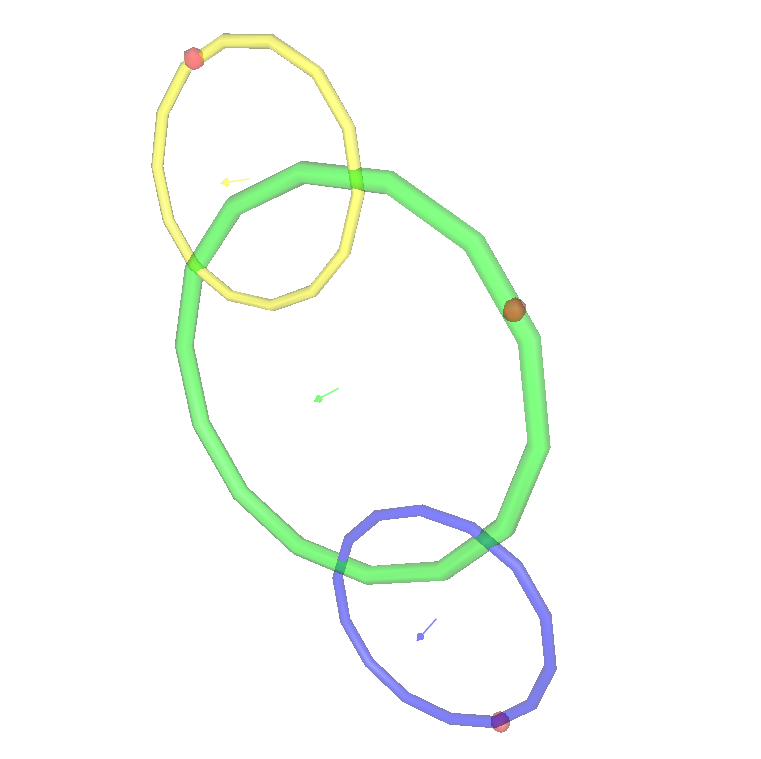
\includegraphics[scale=0.3]{CirclesForEllipseFigure}
\caption{For each circle shown here, the circle is represented by $g(x)$ where $x$ is the point on that circle.
($w$ was chosen so that $v\cdot w\approx\cos 1$.)
If you put a rubber-band around the circles, you can an approximation of an ellipse.  The more circles we have,
the better this approximation.}
\label{fig_circles_of_ellipse}
\end{figure}
Can we recover the characteristics of this ellipse from
the function $g$?  Well,
\begin{equation*}
w=\nvao\wedge\nvai\cdot g(x)\wedge\nvai.
\end{equation*}
If we then let
\begin{equation*}
h(x)=\nvao\wedge\nvai\cdot g(x)\wedge\nvao\wedge\nvai=(x\cdot v)v\wedge w,
\end{equation*}
we then see that $w-\nabla h(x)=(v\cdot w)v$, in which case we can normalize
this vector to recover $v$ up to sign.  We can then recover $r$ as
\begin{equation*}
r = \sqrt{1-2w(\nvao\wedge\nvai\cdot\nvao\wedge g(v))}.
\end{equation*}
Our decomposition is complete.  We can then calculate the larger
diameter of the ellipse as $r(v\cdot w)^{-1}$, the smaller
diameter being $r$, but what good is the function $g$ if we can't
use it to somehow draw the ellipse?  Interestingly, this turns out to be a very
easy and natural thing to do.  Simply notice that the set
\begin{equation*}
\{g(\lambda v)\wedge(v+\lambda\nvai) | \lambda\in[-\alpha,\alpha]\},
\end{equation*}
where $\alpha=r\sqrt{1-(v\cdot w)^{-2}}$, is the set of all blades representative
of point-pairs on the ellipse!  From this we can easily extrapolate all points on the ellipse.
The following figure illustrates a sequence of point-pairs on the same ellipse
shown in figure \ref{fig_circles_of_ellipse}, this time on a different attitude.
\begin{figure}[H]
\centering
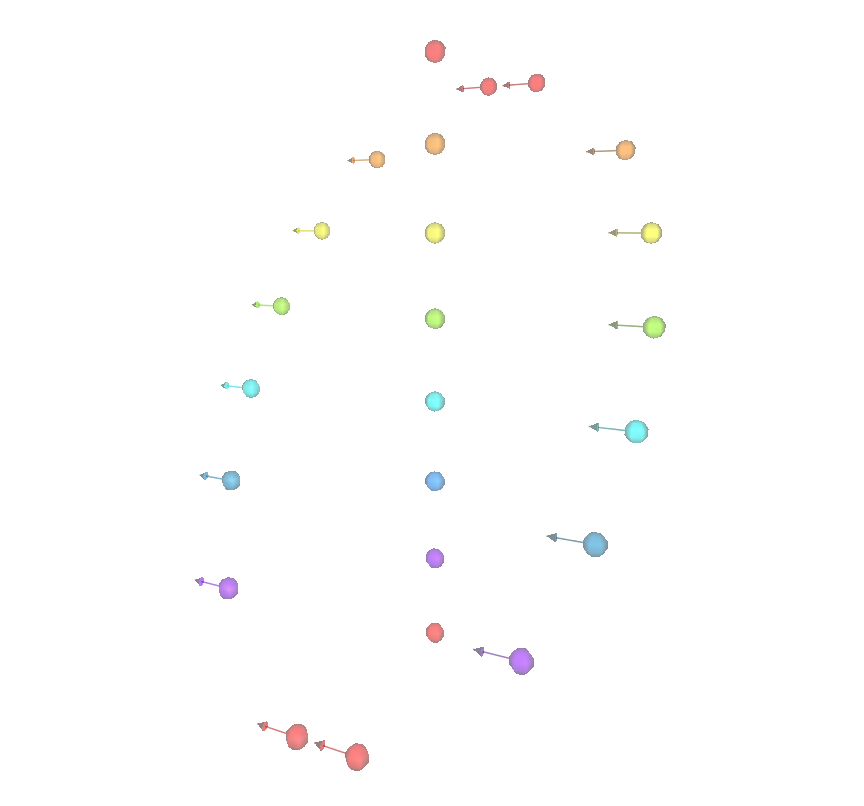
\includegraphics[scale=0.3]{PointPairsForEllipseFigure}
\caption{The dotted out-line of an ellipse made by a sequence of point-pairs.
Here, each point-pair is given the same color as the point $\lambda v$
used in the function $g(x)\wedge(v+(v\cdot x)\nvai)$ used to generate that point-pair.}
\label{fig_circles_of_ellipse}
\end{figure}

From this idea a computer algorithm could be easily created that can
draw these types of ellipses.

\subsection{Reflections With Geometric Functions}

Geometric functions are just mappings from points to blades
representative of traditional conformal geometries.  Furthermore,
since we know by result $\eqref{rslt_reflections_are_geometry}$
that all such blades can be rewritten as a versor, the action of
which is well understood by our recent study of reflections, it then seems natural to ask at this point if reflections about
geometries represented by geometric functions can be accomplished.
In an attempt to answer this question,
it seems reasonable to me that we would define the reflection of a
traditional conformal geometry, (one represented by a constant geometric function),
in a geometry represented by non-constant geometric functions as follows.
\begin{definition}\label{def_geo_func_reflection}
Let $B\in\G$ be dually representative of any conformal geometry,
and let $g:\V^n\to\G$ be a dual geometric function.  Then the geometry
that is the reflection of the geometry represented by $B$ in the
geometry represented by $g$ is given by the set
\begin{equation*}
\{x\in\V^n|\mbox{$\exists y\in\V^n$ such that $p(y)\in B^*$ and $g(y)p(y)g^{-1}(y)=p(x)$}\}.
\end{equation*}
\end{definition}
Thinking about the infinite cylinder given in the previous section, this appears to
make sense.  What we can now show is that if a geometric function has what
we'll call the reflective property, then it is easy to find the geometric function
that represents the reflection of a traditional conformal geometry in a geometry
represented by a geometric function.
\begin{definition}
We say that a geometric function $g$ has the reflective property if for
any $y\in\V^n$, $g(y)=g(x)$, where $x\in\V^n$ and $p(x)=g(y)p(y)g^{-1}(y)$.
\end{definition}
\begin{result}\label{rslt_geo_func_reflect}
Let $g:\V^n\to\G$ be a dual geometric function possessing the reflective property,
and let $B$ be a blade dually representative of any conformal geometry.  Then
the geometric function $r:\V^n\to\G$ given by
\begin{equation*}
r(x) = g(x)Bg^{-1}(x)
\end{equation*}
is dually representative of the reflection of the geometry represented by $B$ about 
the geometry represented by $g$.
\end{result}
\begin{proof}
Let $y\in\V^n$ be any point such that $p(y)\cdot B=0$.  Let $x\in\V^n$
be the point where $p(x)=g(y)p(y)g^{-1}(y)$.  We then have
\begin{align*}
p(x)\cdot r(x) &= [g(y)p(y)g^{-1}(y)]\cdot [g(x)Bg^{-1}(x)] \\
 &= [g(x)p(y)g^{-1}(x)]\cdot[g(x)Bg^{-1}(x)] \\
 &= g(x)[p(y)\cdot B]g^{-1}(x) = 0,
\end{align*}
by the reflective property of $g$ and a lemma I need to come up with.
Suppose now that $x$ is a point such that $p(x)\cdot r(x)=0$.
Let $y$ be the point such that $p(x)=g(y)p(y)g^{-1}(y)$.
It then follows that $g(x)[p(y)\cdot B]g^{-1}(x)=0$, which
implies that $p(y)\cdot B=0$.
\end{proof}

It is easy to show that geometric function in equation $\eqref{equ_cylinder}$ has
the reflective property.  Notice first that for all $x\in\V^n$, that $g(x)$ is dually
representative of a sphere centered at $y=c+((x-c)\cdot v)v$.  Then realizing that any spherical
reflection of $x$ in this sphere will move it along a line containing $x$ and $y$,
we need only show that $g(x)=g(\lambda y+(1-\lambda )x)$ for any $\lambda\in\R$.
Indeed, as the reader can check, we have
\begin{equation*}
c+((\lambda y+(1-\lambda)x-c)\cdot v)v = c+((x-c)\cdot v)v.
\end{equation*}
We can now conclude by result $\eqref{rslt_geo_func_reflect}$ that the notion of reflectance given in
definition $\eqref{def_geo_func_reflection}$ is represented
by the geometric function $g(x)Bg^{-1}(x)$.  The question now is: given a
blade $B$ representative of certain geometries, how can we relate this
geometric function to one in a canonical form?  Without such a relation,
we can't make much use of our geometric function in terms of deciphering
the characteristics of the geometry it represents.

Go on...

\section{Concluding Remarks}

This introduction has only just begun to scratched the surface of
what kinds of geometry we can do with the conformal model, and
any model like it that uses a homogeneous blade representation scheme,
such as the model for projective geometry.  It is reasonable to ask
what other models of geometry there might be that use different
types of geometric algebras.  Instead of going in search of a model
with specific features, we might as well just choose a geometric algebra,
and then ask what types of geometry we can do with that algebra under
various models of geometry.

One of the main features of this paper has been the idea in my mind
that the conformal model is just pure Euclidean geometry, and while
it is implemented in a non-Euclidean geometric algebra, there is no
need to give proofs with geometric arguments that require the reader
to visualize projective space.  In fact, I will go so far as to say that
I have never liked the terms null vector at infinity and null vector at
the origin.  To me, the only difference between these two vectors, which are algebraically identical,
is how we use them in the model, and I almost wouldn't mind calling them null vector zero
and null vector one.\footnote{Almost, because I must admit that there really is some intuition to
be gained about geometry in the conformal model in thinking of $\nvao$ as an origin and $\nvai$ as a point at infinity.}
In my mind, the model simply uses the algebraic properties
of the underlying non-Euclidean geometric algebra, (lemmas, theorems, results, etc.), as logical tools for
solving problems in Euclidean geometry.  I have never tried too hard to visualize the vectors in the geometric
algebra $\G(\V)$, but only the vectors and blades in the geometric algebra $\G(\V^n)$.

It should also be observed, I believe, that there are note-worthy similarities in the
development of the conformal model with that of algebraic geometry.
It is my guess that algebraic geometry is more general in its
ability to answer geometric questions and in its breadth of geometric representation.
Could the concepts of geometric algebra be brought to bare in answering the questions of algebraic
geometry?  Is there a reformulation of algebraic geometry in terms of geometric algebra?
Would this expand and enrich the subject?  I do not know.  All I really do know is
that doing geometry with conformal geometric algebra is a lot of fun!

\pagebreak
\bibliographystyle{plain}
\bibliography{CGAIntro}

\end{document}

% How does meet and join perform operations on geometry in the conformal model?